\documentclass[10pt,letterpaper]{article}
\usepackage{aaai}
\usepackage{xparse}
\usepackage{times}
\usepackage{helvet}
\usepackage{courier}
\usepackage{tabularx}
\usepackage{amsmath}
\usepackage{amssymb}
\usepackage{xspace}
\usepackage{relsize}
\usepackage{aaai_my}
\usepackage{graphicx}
\usepackage{abbrev}
\usepackage{multirow}
\usepackage{xr}
\usepackage{pdflscape}
\usepackage{bm}
\externaldocument{asai}
\renewcommand{\thesection}{S\arabic{section}}
\renewcommand{\thetable}{S\arabic{table}}
\renewcommand{\thefigure}{S\arabic{figure}}
\newcommand{\argmin}{\mathop{\rm argmin}}
\newcommand{\argmax}{\mathop{\rm argmax}}
\newcommand{\bx}{\mathbf{x}}
\newcommand{\bz}{\mathbf{z}}
\newcommand{\bb}{\mathbf{b}}
% \usepackage[margin=1cm]{geometry}

\setlength{\pdfpagewidth}{8.5in}
\setlength{\pdfpageheight}{11in}
\pagestyle{empty}
\frenchspacing
\setcounter{secnumdepth}{2}
% \setlength{\floatsep}{1mm}
% \setlength{\textfloatsep}{1mm}
% \setlength{\abovecaptionskip}{1mm}
% \setlength{\belowcaptionskip}{1mm}
% \setlength{\abovedisplayskip}{1mm}
% \setlength{\belowdisplayskip}{1mm}
% \setlength{\arraycolsep}{0.5mm}
% \setlength{\tabcolsep}{0.1em}


\nocopyright
\author{Supplemental materials for Paper ID: 4597}
\title{Don't Cry Wolf! : Towards Stable Symbol Grounding\\ with Zero-Suppressed State AutoEncoder}
\begin{document}
\maketitle

\section{Gumbel-softmax Variational Autoencoder}
\label{gumbel-softmax-theory}
This section reviews the Gumbel-softmax variational autoencoder~(GS-VAE), and its connection to the entropy regularization.

\subsection{Objective Function of Variational Autoencoder~(VAE)}
We first derive the learning algorithm of VAE when the latnet representation is a binary vector.
Assume that we have a data set, $\mathcal{X}=\{\mathbf{x}^{(1)},\dots,\mathbf{x}^{(I)}\}$.
The first objective of VAE is to obtain a probability distribution that well explains $\mathcal{X}$.
In other words, letting $\{p(\mathbf{x};\theta) \mid \theta\in\Theta\}$ be a family of parametric probability distributions, we wish to obtain,
\begin{align*}
\theta^\star = \argmax_{\theta\in\Theta} \prod_{\mathbf{x}\in \mathcal{X}} p(\mathbf{x};\theta)
\end{align*}
which maximize the probability that such a dataset is obtained. Since a product is hard to compute, we instead maximize the log-probability, i.e.
\begin{align*}
\theta^\star = \argmax_{\theta\in\Theta} \sum_{\mathbf{x}\in \mathcal{X}} \log p(\mathbf{x};\theta).
\end{align*}
as $\log$ preserves the maxima.
In practice, we instead optimize for the minimization objective, hence we get a equivalent formulation
\begin{align*}
\theta^\star = \argmin_{\theta\in\Theta} - \sum_{\mathbf{x}\in \mathcal{X}} \log p(\mathbf{x};\theta).
\end{align*}


A key assumption we have now is that the probability distribution has a $N$-dimensional latent variable $\mathbf{b}=\parens{b_n}\in\{0,1\}^N$, which is not observable.
By the basic sum rule of marginal probability,
$p(\mathbf{x};\theta) = \sum_{\mathbf{b}\in\{0,1\}^N}p(\mathbf{x}, \mathbf{b};\theta)$ holds, and further,
by the basic chain rule,
$p(\mathbf{x}, \mathbf{b};\theta) = p(\mathbf{x} \mid \mathbf{b};\theta)p(\mathbf{b})$ holds.
Therefore the objective boils down to,
\begin{align}
\label{eq:vae-obj} \theta^\star = \argmin_{\theta\in\Theta} -\sum_{\mathbf{x}\in \mathcal{X}} \log \left(\sum_{\mathbf{b}\in\{0,1\}^N}p(\mathbf{x} \mid \mathbf{b};\theta)p(\mathbf{b})\right).
\end{align}

The encoder-decoder structure appears by the variational approximation.
Let $q(\mathbf{b} \mid \mathbf{x};\phi)$ be a variational distribution which approximates $p(\mathbf{b} \mid \mathbf{x};\theta)$, the probability of getting $\mathbf{b}$ given $\mathbf{x}$, which is unknown because $\mathbf{b}$ is not observable.
With $q$, the summand of the objective function of Eq.~\eqref{eq:vae-obj} is upper-bounded as follows:
\begin{align}
\nonumber & - \log \left(\sum_{\mathbf{b}\in\{0,1\}^N} p(\mathbf{x} \mid \mathbf{b};\theta)p(\mathbf{b})\right) \\
\nonumber = & -  \log \left(\sum_{\mathbf{b}\in\{0,1\}^N}\dfrac{p(\mathbf{x} \mid \mathbf{b};\theta) p(\mathbf{b})}{q(\mathbf{b} \mid \mathbf{x}; \phi)}q(\mathbf{b} \mid \mathbf{x}; \phi)\right)\\
%\label{eq:vae-q-exp}
\nonumber\leq & - \sum_{\mathbf{b}\in\{0,1\}^N} q(\mathbf{b} \mid \mathbf{x}; \phi)\log \left(\dfrac{p(\mathbf{x} \mid \mathbf{b};\theta) p(\mathbf{b})}{q(\mathbf{b} \mid \mathbf{x}; \phi)}\right)\\
\nonumber =   &   \sum_{\mathbf{b}\in\{0,1\}^N} q(\mathbf{b} \mid \mathbf{x}; \phi) \left(-\log p(\mathbf{x} \mid \mathbf{b};\theta) \right)\\
\nonumber     & - \sum_{\mathbf{b}\in\{0,1\}^N} q(\mathbf{b} \mid \mathbf{x}; \phi)\log \left(\dfrac{p(\mathbf{b})}{q(\mathbf{b} \mid \mathbf{x}; \phi)}\right) \\
\label{eq:vae-obj-final}= & \mathbb{E}_{q(\mathbf{b} \mid \mathbf{x}; \phi)}[-\log p(\mathbf{x} \mid \mathbf{b};\theta)] + \mathrm{KL}(q(\mathbf{b} \mid \mathbf{x}; \phi) || p(\mathbf{b})),
\end{align}
resulting in the objective function of VAE~(Eq.~\eqref{eq:vae-obj-final}).
The inequality is due to Jensen's inequality.
In the above expression, $q(\mathbf{b} \mid \mathbf{x};\phi)$ can be regarded as the encoder, and $p(\mathbf{x}\mid \mathbf{b};\theta)$ can be regarded as the decoder.
%By further investigating Eq.~\eqref{eq:vae-q-exp}, since $q$ is factorized into $N$ distributions, 

%% this assumption is not relevant at the moment.
For $q$, we also assume each axis $b_n$ in $\mathbf{b}$ are mutually independent, i.e. $q(\mathbf{b} \mid \mathbf{x};\phi)=\prod_{n=1}^N q(b_n \mid \mathbf{x};\phi_n)$,
in order to make the later computation easier.


\subsection{Reparametrization Trick}
When learning model parameters $\theta$ and $\phi$, we usually rely on stochastic gradient descent~(SGD), rather than computing the gradient over all of the data points.
In the case of VAE, not only the data point $\mathbf{x}\in \mathcal{X}$, but also the latent vector $\mathbf{b}$ is sampled using $q$ in order to compute the per-example loss without taking the expectation over $\mathbf{b} \in \braces{0,1}^N$, which is exponentially large.
The reparameterization trick allows us to apply a stochastic approximation to the latent vector.
Its main idea is to decompose the random variable $\mathbf{b}$ into a deterministic and parameterized part~(thus, dependent on $\phi$) and a random and non-parameterized part~(thus, independent from $\phi$).
Such a decomposition yields a following repetitive algorithm:
\begin{enumerate}
 \item Sample $\mathbf{x}$ from $\mathcal{X}$.
\item Sample $\mathbf{b}$ using $q(\mathbf{b} \mid \mathbf{x} ;\phi)$. (The sampling methods is specified later.)
 \item Compute the gradients of,
       \begin{align}
	\label{eq:stochastic-approx}
	-\log p(\mathbf{x} \mid \mathbf{b};\theta) - \log\left(\frac{p(\mathbf{b})}{q(\mathbf{b} \mid \mathbf{x};\phi)}\right),
       \end{align}
       with respect to $\theta$ and $\phi$.
 \item Update $\theta$ and $\phi$ using the gradients.
\end{enumerate}

\subsection{Gumbel-softmax Variational Autoencoder}
In the case of binary latent representations, a Gumbel-softmax distribution~(which is also known as a concrete distribution) is used to apply the reparameterization trick.
The Gumbel-softmax distribution is a continuous relaxation of the Bernoulli distribution, and therefore,
a random variable following the Gumbel-softmax distribution resides in $[0,1]$, rather than $\{0,1\}$.
The accuracy of approximation is controlled by a temperature parameter $\tau\in(0,\infty)$.
The lower the temperature is, the closer the Gumbel-softmax distribution is to the Bernoulli distribution.
In specific, let $\bm{\pi}=\begin{bmatrix}\pi_0 & \pi_1\end{bmatrix}$ be the unnormalized logit parameter of the Gumbel-softmax distribution.
As $\tau\rightarrow 0$, the Gumbel-softmax distribution becomes the Bernoulli distribution of parameter $\pi_1/(\pi_0 + \pi_1)$.
Let $q(\bz \mid \bx;\bm{\pi},\tau)$ be the decoder using the Gumbel-softmax distribution.

When replacing the binary random variable $\mathbf{b}\in\{0,1\}^N$ with the continuous random variable $\mathbf{z}\in[0,1]^N$, we apply the following approximations.
For the decoder, we directly plug-in its continuous relaxation $\bz$ to the decoder to obtain $p(\bx \mid \bz;\theta)$.
The reconstruction loss term in Eq.~\eqref{eq:vae-obj-final} is approximated by substituting the Gumbel-softmax distribution $q(\bz \mid \bx;\phi,\tau)$ for the Bernoulli distribution $q(\bb \mid \bx;\phi)$.
The KL term in Eq.~\eqref{eq:vae-obj-final} is approximated by substituting $q(\bz \mid \bx;\bm{\pi},\tau=0)$ for $q(\bb \mid \bx;\phi)$.
The KL divergence is still well-defined because the Gumbel-softmax distribution now coincides with the Bernoulli distribution.
Since the KL term is defined over Bernoulli distributions, the same discussion as that made in Section~\ref{analysis} can be applied.


\section{Implementation Details}

\subsection{Computing Gumbel-Softmax}
\label{gumbel-softmax-implementation}

Given that the theoretical background of Gumbel-softmax fully specified, we now proceed to introduce the
more down-to-earth implementation details of Gumbel-softmax.

% Since the random distribution is not differentiable (BP is not applicable), VAEs use \emph{reparameterization tricks}, which decompose the target distribution into a differentiable and a purely random distribution (the latter does not require the gradient).
% For example, the Gaussian $N(\sigma,\mu)$ is decomposed to $\mu+\sigma N(1,0)$, where $\mu,\sigma$ are learned.
% In addition to the reconstruction loss, VAE should also minimize the variational loss (the difference between the learned and the target distributions) measured by, e.g.,  KL divergence.

% Gumbel-Softmax (GS) is a reparametrization trick \cite{jang2016categorical} for categorical distribution.
% It continuously approximates Gumbel-Max \cite{maddison2014sampling}, a method for drawing categorical samples.
Assume the output $\mathbf{z}=(z_i)$ is a one-hot vector, e.g.,
% if the domain is $D=\braces{a,b,c}$, then $\mathbf{z}=\parens{0,1,0}$ represents ``b'',
if the domain is $D=\braces{false,true}$, then $\mathbf{z}=\parens{0,1}$ represents ``true''.
% The input is a class probability vector $\pi$, e.g. $\parens{.1,.1,.8}$.
The input is a class probability vector $\pi$, e.g. $\parens{.2,.8}$.
While in our paper we always use the binary categories
for we aim to represent the input in a binary vector,
Gumbel-softmax itself easily extends to more than two classes such as $D=\braces{a,b,c}$
and therefore, in this section, we describe the general case as in the original paper \cite{jang2016categorical}.

We first describe a related method for drawing a categorical sample from $\pi$, Gumbel-Max technique \cite{maddison2014sampling}.
It is a generalization
of the method for drawing a boolean sample from a Bernoulli distribution with parameter $\pi_1/(\pi_0 + \pi_1)$.
Gumbel-Max draws samples from $D$ with the following function:
\[
z_i \equiv [ \text{if}\ i\ \text{is} \arg \max_i (g_i+\log \pi_i) \text{then}\ 1\ \text{else}\ 0 ]
\]
where $g_i$ are i.i.d samples drawn from
 $\text{Gumbel}(0,1) =-\log (-\log u)$ \cite{gumbel1954statistical}, where
$u$ is a uniform random sample between 0 and 1.
Gumbel-Softmax approximates argmax with softmax to make it differentiable:
\[
z_i = \text{Softmax}((g_i+\log \pi_i)/\tau).
\]
``Temperature'' $\tau$ controls the magnitude of approximation, which is annealed to 0 by a certain schedule.
The output $\mathbf{z}$ converges to a discrete one-hot vector when $\tau\approx 0$.

In SAEs, we have $N$ gumbel-softmax units of $|D|=2$ categories ($D=\braces{\text{true},\text{false}}$)
to model an $N$-dimensional Bernoulli/boolean/propositional variable $\mathbf{b}=(b_n)$.
Thus the latent layer is a matrix $z_{nk}$ rather than a vector, where $1\leq n \leq N$ and $k\in\braces{0,1}$.
The actual boolean (Bernoulli / propositional) variable is then retrieved by $b_n=z_{n1}$.




\subsection{Removing Stochasticity from Gumbel-Softmax during Run-Time}
\label{argmax-implementation}
% Another observation we made from the source code is that we can
% disable the runtime stochasticity of the network.
We can disable the runtime stochasticity of the network that contains Gumbel-Softmax.
After the training is finished, we replace the gumbel-softmax activation with
a pure argmax of class probabilities:
\[
 z_{nk} = [ \text{if}\ k\ \text{is} \arg \max_k (\log \pi_{nk})\ \text{then}\ 1\ \text{else}\ 0 ].
\]
% 
This technique reduces the inherent stochasticity of the network
but does not reduce the stochasticity originated from the noisy input.
% Recall that $Q(D|x)$ is a conditional distribution defined for a single, \emph{fixed} input $x$.
% % 
% For instance, the propositional representation may be altered by a small
% Gaussian noise applied to the input.

\subsection{Zero-Suppression Implementation}
\label{zsae-implementation}
In the actual implementation of zero-suppression regularization,
$b_n$ corresponds to the value in the activation matrix $z_{n1}$.
Thus we sum them up instead.

\subsection{Pruning the Zero-Suppressed Network Node}
\label{pruning-implementation}

Assume the propositional layer $z_{nk}$ is connected to the next layer of $L$ neurons
by a fully-connected network $h_l=\sigma\parens{\sum_{nk} W_{nkl}z_{nk}+B_l}$
with weights $W_{nkl}$ and biases $B_l$.
When we assume that $z_{n0}=1,z_{n1}=0$ always holds ($b_n=0$ for all inputs),
we can prune the index $n$
by adding $W_{n0l}$ to $B_l$ and removing $W_{nkl}$ for $\forall k\in\braces{0,1}$, $\forall l \in [1..L]$,
which removes $2L$ float values for each zero-suppressed bit $b_n$.
Therefore, if we remove $\Delta N$ bits from the latent space, it removes $2L\Delta N$ float values from the network.
 
We can similarly prune the weights $W'$ from the previous layer of $M$ neurons.
When $W'=(W'_{mnk})$ and bias $B'=(B'_{nk})$ ($m\in[1..M], n\in[1..N], k\in \braces{0,1}$),
we remove $2(M+1)$ for each zero-suppressed bit $b_n$.
Therefore, if we remove $\Delta N$ bits from the latent space, it removes $2(M+1)\Delta N$ float values from the network.

\subsection{Network Size}
\label{network-implementation}
All of the SAE networks used in the evaluation have the same network
topology for each domain, except the input layer which should fit the size of the input
images, the zero-suppression coefficient $\alpha$ and the latent layer size $N$.
They are implemented with TensorFlow and Keras libraries.
All layers except Gumbel-Softmax in the network are the very basic ones introduced in a standard tutorial.

The network uses convolutional layers in the encoder, and fc layers
in the decoder (\refig{fig:sae-detail}).
Input layer has the same dimension as the image size.
The network was trained by the Adam optimizer \cite{kingma2014adam}.
In all domains, we used 150 epochs, batch-size 1000 and the learning rate 0.001.

\begin{figure}[htb]
\centering
\begin{tabular}{|l|}
 Input($input$),\\
 GaussianNoise(0.4),\\
 conv(3,3,16), tanh, bn, dropout(0.4),\\
 conv(3,3,16), tanh, bn, dropout(0.4),\\
 fc(2$N$), reshape($N\times 2$), GumbelSoftmax,\\
 fc(1000), relu, bn, dropout(0.4),\\
 fc(1000), relu, bn, dropout(0.4),\\
 fc($input$), sigmoid.
\end{tabular}
\caption{SAE implementation.
 Here, fc = fully connected layer, conv = convolutional layer, 
relu = Rectified Linear Unit,
bn = Batch Normalization, % \cite{ioffe2015batch} ,
and tensors are reshaped accordingly.}
\label{fig:sae-detail}
\end{figure}

% The last layers can be replaced with [fc($input\times 2$), GumbelSoftmax, TakeFirstRow]
% for better reconstruction when we can assume that the input image is binarized.

In all experiments, 
the annealing schedule of Gumbel-Softmax is $\tau \leftarrow \max (0.7, \tau_0\exp(-rt))$ where
 $t$ is the current training epoch, $\tau_0$ is the initial temperature and $r$ is an annealing ratio.
We chose $\tau_0,r$ so that $\tau = 5.0$ when the training starts and $\tau = 0.7$ when the training finishes.
The above schedule is similar to the original schedule in  \citeauthor{jang2016categorical} (\citeyear{jang2016categorical}).



\section{Supplemental Experiments}


\subsection{State Variance without Replacing GS with Argmax}

We measured the state variance while keeping the inherent network stochasticity,
i.e., without the argmax techniques to
make the network deterministic (\refsec{argmax}, \refsec{argmax-implementation}).

\begin{table}[htbp]
 \relsize{-1.5}
 \centering
 \setlength{\tabcolsep}{0.45em}
 \begin{tabular}{|r|*{4}{c|}}
       & \multicolumn{4}{c|}{Mean variance over bits} \\
$N=$ % & \multicolumn{2}{c|}{36} 
     % & \multicolumn{2}{c|}{64}
     & \multicolumn{2}{c|}{100}
     & \multicolumn{2}{c|}{1000} \\
  % data for N=36
% &SAE      &ZSAE     
% &0.00E+00 &3.44E-03 
% &4.69E-05 &6.25E-07 
% &6.25E-07 &2.92E-06 
% &7.03E-05 &5.30E-03 
% &6.17E-04 &4.81E-03 
  % data for N=64
% &SAE      &ZSAE     
% &2.20E-04 &1.05E-06 
% &1.82E-04 &0.00E+00 
% &8.10E-05 &0.00E+00 
% &1.50E-03 &5.84E-04 
% &1.36E-04 &1.00E-04 
domain   &SAE      &ZSAE     &SAE      &ZSAE     \\ 
MNIST    &3.92E-04 &0.00E+00 &1.18E-04 &1.33E-08 \\ 
Mandrill &1.51E-04 &0.00E+00 &6.13E-05 &2.60E-07 \\ 
Spider   &9.73E-05 &2.25E-07 &4.82E-05 &7.88E-06 \\ 
LightsOut&7.81E-05 &1.36E-05 &4.23E-04 &7.95E-06 \\ 
Twisted  &5.51E-04 &2.12E-05 &6.39E-04 &5.47E-03 \\ 
\end{tabular}
 \caption{Results comparing the state variance of vanilla SAE and ZSAE ($\alpha=0.7$),
 over 100 randomly generated images encoded 100 times (no noise is added each time).
 ZSAE suppresses the state variance, but not to absolute zero.
 }
\label{tab:variance-stochastic}
\end{table}

We randomly generated 100 images with a domain-specific generator for each puzzle domain,
then encoded each of them with the SAE 100 times.
We measured the variance of the propositions, i.e. the variance of the latent activations (0 or 1)
across 100 encoding trials of the same image.
We then took the mean of the variances over the entire propositions.

The results indicate that ZSAE also suppresses the effect of internal stochasticity.
We do not include these results to the main paper due to space,
and also the argmax technique (\refsec{argmax}, \refsec{argmax-implementation})
completely eliminates the internal stochasticity.
However, the argmax technique only reduces the inherent stochasticity of the network
and not the stochasticity originated from the noisy input.
Therefore, ZSAE is still necessary when the input is noisy (which is the case in almost all real-world scenario),
as discussed in the main paper.

When we enable the argmax technique, the state variances for noiseless input become 0 for all networks.

\subsection{The percentage of true propositions}

\begin{table}[htbp]
 \relsize{-1.5}
 \centering
 \setlength{\tabcolsep}{0.45em}
 \begin{tabular}{|r|*{4}{c|}}
       & \multicolumn{4}{c|}{True ratio} \\
$N=$ & \multicolumn{2}{c|}{100} & \multicolumn{2}{c|}{1000} \\
domain    & SAE  & ZSAE & SAE  & ZSAE \\ 
MNIST     & 0.50 & 0.10 & 0.50 & 0.02 \\ 
Mandrill  & 0.50 & 0.12 & 0.50 & 0.09 \\ 
Spider    & 0.50 & 0.14 & 0.50 & 0.11 \\ 
LightsOut & 0.50 & 0.08 & 0.50 & 0.03 \\ 
Twisted   & 0.50 & 0.08 & 0.50 & 0.02 \\ 
\end{tabular}
 \caption{Results comparing the characteristics of vanilla SAE and ZSAE ($\alpha=0.7$),
 over 100 randomly generated images encoded 100 times (with gaussian noise added each time).
 }
\label{tab:trueratio}
\end{table}

We measured the average percentage of propositions that turned true on ZSAE/SAE.
\reftbl{tab:trueratio} shows that the ratio significantly drops due to the Zero-suppression penalty,
demonstrating that $p_a(\mathbf{b})$ (\refsec{analysis}) is altered by the regularization.

\subsection{MSE and Effective Bits for different $\alpha$}
\label{more-sensitivity}

\begin{table}[htbp]
 \relsize{-1.5}
 \centering
 \setlength{\tabcolsep}{0.25em}
 \begin{tabular}{|r|*{8}{c|}}
     & \multicolumn{8}{c|}{Mean Square Error} \\
$N=$ & \multicolumn{4}{c|}{100} & \multicolumn{4}{c|}{1000} \\
     & SAE & \multicolumn{3}{c|}{ZSAE} & SAE & \multicolumn{3}{c|}{ZSAE} \\
domain    &   & $\alpha$=0.2 & 0.5  & 0.7 &   & $\alpha$=0.2 & 0.5  & 0.7 \\ 
MNIST     & 1.9E-7  &5.9E-8 & 3.4E-7 & 2.9E-6 &8.3E-11 &9.6E-7  & 8.9E-11 &3.2E-10 \\ 
Mandrill  & 3.0E-4  &2.4E-4 & 2.7E-4 & 2.8E-4 &2.1E-4  &2.9E-4  & 2.3E-4  &2.3E-4  \\ 
Spider    & 2.7E-4  &2.5E-4 & 1.9E-4 & 2.2E-4 &3.1E-4  &5.5E-4  & 2.8E-4  &2.8E-4  \\ 
LightsOut & 2.8E-14 &9.7E-5 & 2.6E-5 & 1.2E-5 &1.5E-14 &3.9E-14 & 2.3E-14 &8.0E-6  \\ 
Twisted   & 4.8E-5  &6.9E-5 & 5.0E-5 & 5.1E-5 &8.4E-5  &5.6E-5  & 6.9E-5  &4.5E-5  \\
  % 
\multicolumn{9}{c}{}\\
  % 
     & \multicolumn{8}{c|}{Effective Bits} \\
$N=$ & \multicolumn{4}{c|}{100} & \multicolumn{4}{c|}{1000} \\
     & SAE & \multicolumn{3}{c|}{ZSAE} & SAE & \multicolumn{3}{c|}{ZSAE} \\
domain    &   & $\alpha$=0.2 & 0.5  & 0.7 &   & $\alpha$=0.2 & 0.5  & 0.7 \\ 
MNIST     & 100 & 50 & 51 & 46 & 1000 & 72  & 55  & 62  \\ 
Mandrill  & 100 & 69 & 50 & 47 & 1000 & 868 & 673 & 164 \\ 
Spider    & 100 & 81 & 50 & 48 & 1000 & 794 & 356 & 85  \\ 
LightsOut & 100 & 54 & 19 & 17 & 1000 & 431 & 154 & 76  \\ 
Twisted   & 100 & 40 & 17 & 16 & 1000 & 973 & 68  & 43  \\ 
\end{tabular}
 \caption{
MSE sensitivity of ZSAE to the hyperparameter $\alpha$ is low.
Similarly,
the number of effective bits is not sensitive to the hyperparameter $\alpha$ of ZSAE.
}
\label{tab:more-sensitivity}
\end{table}

\clearpage
\section{Plan Execution Examples}

\begin{figure}[h]
 \centering
 (1)
 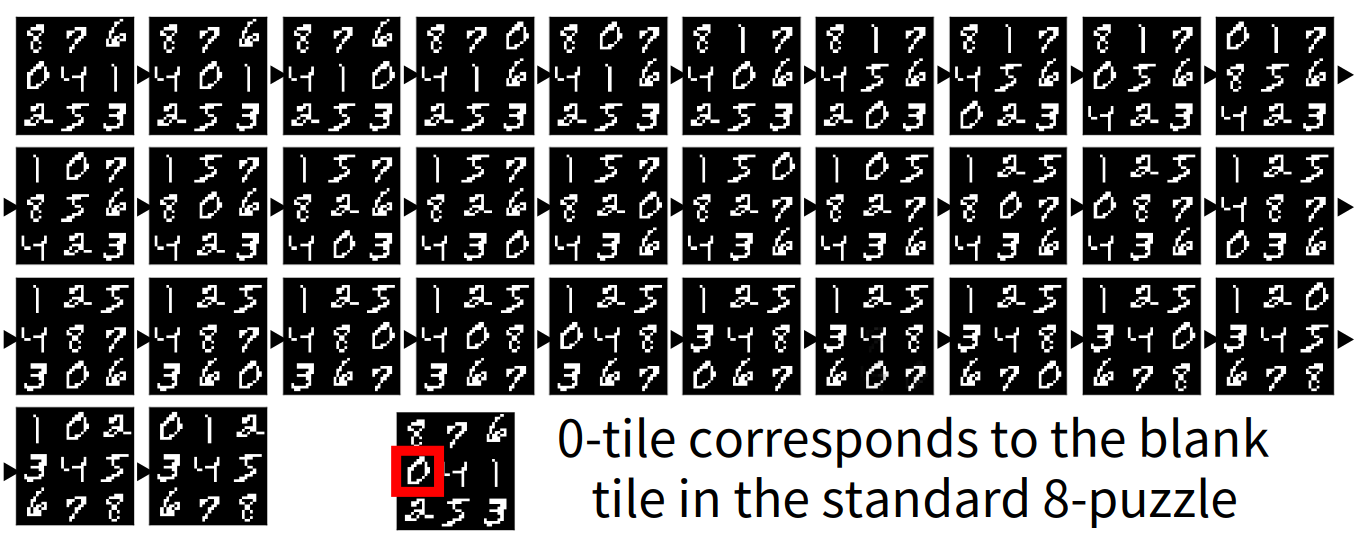
\includegraphics[width=0.9\linewidth]{img/mnist-plan-new.pdf}
 (2)
 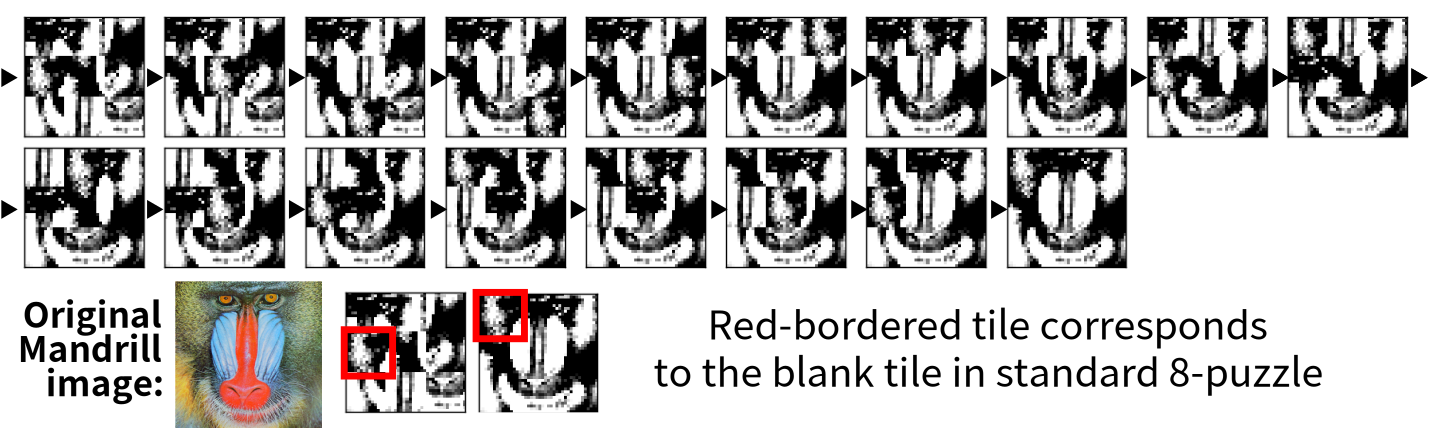
\includegraphics[width=0.9\linewidth]{img/mandrill-plan-new.pdf}
 (3)
 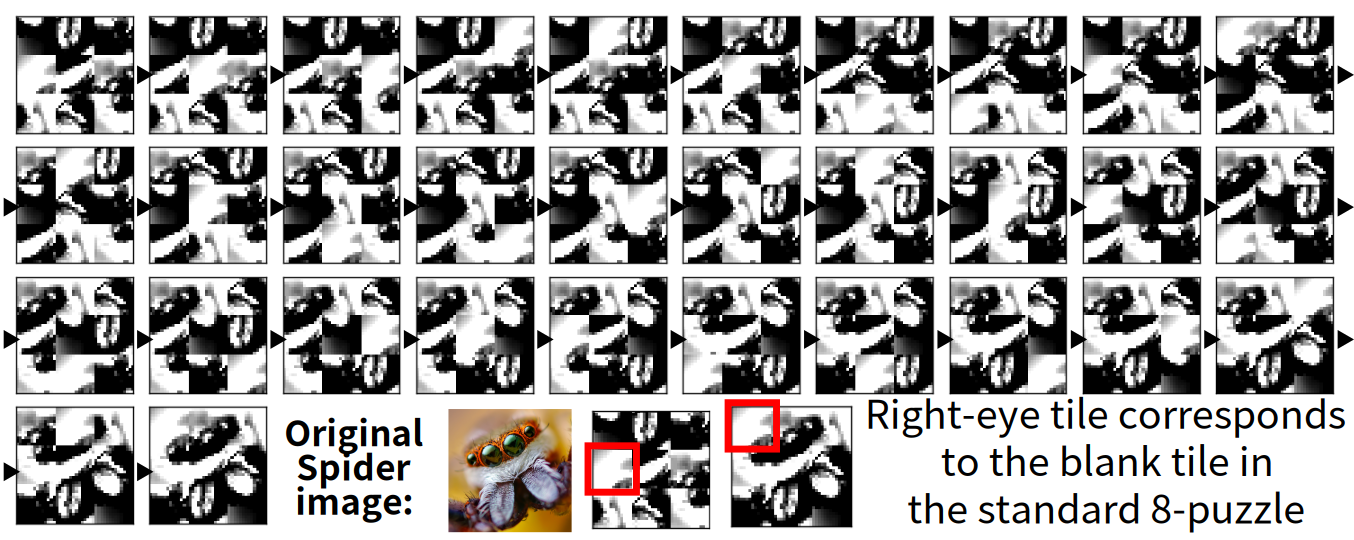
\includegraphics[width=0.9\linewidth]{img/spider-plan-new.pdf}
 (4)
 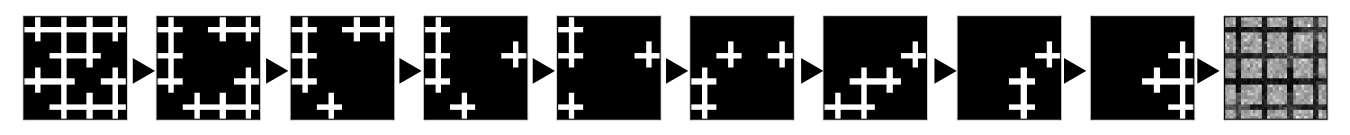
\includegraphics[width=0.9\linewidth]{img/lightsout_new4x4.pdf}
 (5)
 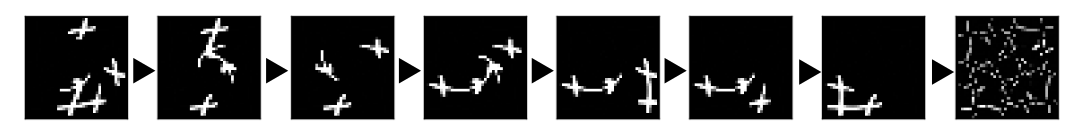
\includegraphics[width=0.9\linewidth]{img/lightsout_twisted_new4x4.pdf}
 \caption{
(1-3)
Output of \latentplanner + AMA$_1$ solving the MNIST/Mandrill/Spider 8-puzzle instance
with the longest (31 steps) optimal plan (Reinefeld 1993).
This shows that \latentplanner finds an optimal solution
given a correct model by AMA$_1$ and an admissible search algorithm.
\latentplanner has no notion of ``slide'' or ``tiles'',
making MNIST, Mandrill and Spider entirely distinct domains.
SAEs are trained from scratch without knowledge transfer.
(4-5) Output of solving 4x4 LightsOut and Twisted LightsOut.
The blurs in the goal states are simply the noise that was normalized and enhanced by the plotting library.
}
 \label{fig:mnist}
\end{figure}

\clearpage
\section{Supplemental Backgrounds}

\subsection{AMA$_1$, an Oracular Action Model Acquisition method}

Action Model Acquisition method AMA$_1$ produces a PDDL/SAS model compatible to
FastDownward \cite{Helmert04}, but is an oracular model which requires the entire state transitions
in the environment.
For each pair of observations $\parens{\before_i, \after_i}$ in the entire set of state transitions allowed in the environment,
AMA$_1$ uses SAE to encodes it into 
a symbolic transition $(Encode(\before_i),$ $Encode(\after_i))=$ $(s_i,t_i)$ where $s_i,t_i$ are propositional states.
Each state (either $s_i,t_i$) is represented as a binary vector $(b_n)_{1\leq n \leq N}$.
Each symbolic transition is then encoded into a PDDL action 
using $s_i$ as its preconditions and the difference of $s_i$ and $t_i$ as its effects.
Each bit $b_n$ is converted into zero-ary predicate \texttt{($b_n$-true)} and \texttt{($b_n$-false)}
when $b_n=1$ and $0$, respectively.
For instance, when $b_5$ is 0 in $s_i$ and 1 in $t_i$,
the preconditions include \texttt{(b5-false)} and
the effects include \texttt{(and (not (b5-false)) (b5-true))}.

\subsection{AMA$_2$: Action Symbol Grounding}
\label{sec:ama2-overview}

\latentplanner + AMA$_1$ shows that (1) the SAE can robustly learn image
$\leftrightarrow$ propositional vector mappings from examples, and that
(2) if all valid image-image transitions (i.e., the entire state space)
is given, \latentplanner can correctly generate optimal plans.  However,
AMA$_1$ is clearly not practical due to the requirement that it uses the
entire state space as input, and lacks the ability to learn/generalize
an action model from a small subset of valid action transitions (image
pairs).  In this section we describe AMA$_2$ \cite{Asai2018}, a neural
architecture which jointly grounds the action symbols and acquires the
action model from the subset of examples, in an unsupervised manner.
AMA$_2$ is approximating AMA$_1$ by learning from examples.

Acquiring a descriptive action model (e.g., PDDL) from a set of unlabeled propositional state transitions consists of three steps.
% 
(Step 1) Identify the ``types'' of transitions, where each ``type'' is an identifiable, \emph{action symbol}.
For example, a  hand-coded ``slide-up-8-at-1-2'' in 8-puzzle is an example of action symbols, but note that an AMA system should ground anonymous symbols without human-provided labels.
% 
While they are not lifted/parameterized, they still provide abstraction. For example, the same ``slide-up-8-at-1-2'' action, which slides the tile 8 at position $(x,y)=(1,2)$ upward, applies to many states (each state being a permutation of tiles 1-7).
% 
(Step 2) Identify the preconditions and the effects of each action and store the information in an action model.
(Step 3) Represent the model in a modeling language (e.g., PDDL).

Addressing this entire process is a daunting task. 
Existing AMA methods typically handle only Steps 2 and 3, skipping Step 1.
Without step 1, however, an agent lacks the ability to learn in an unknown environment where it does not know \emph{what is even possible}.
Note that even if the agent has the full knowledge of its low-level actuator capabilities, it does not know its own high-level capabilities e.g. sliding a tile.
Note that AMA$_1$ handles only Step 3, as providing all valid transitions is equivalent to skipping Step 1/2.

On the other hand, search on a state space graph in an unknown environment is \textit{feasible} even if Step 3 is missing.
PDDL provides two elements, a \emph{successor function} and its \emph{description}.
While ideally both are available, the description is not the \emph{essential} requirement.
The description may increase the explainability of the system in a language such as PDDL,
but such explainability may be lost anyway when the propositional symbols are identified by SAE, as the meanings of such propositions are unclear to humans.
The description is also useful for constructing the heuristic functions, but
the recent success of simulator-based planning \cite{frances2017purely}
shows that, in some application, efficient search is possible without action descriptions.
 
AMA$_2$ thus focuses on Steps 1 and 2.
It grounds the action symbols (Step 1) and finds a successor function that can be used for forward state space search (Step 2), but maintains its implicit representation.
% 
AMA$_2$ comprises two networks: an \emph{Action Autoencoder} (AAE) and an \emph{Action Discriminator} (AD). The AAE jointly learns the action symbols and the action effects, and provides the ability to enumerate the candidates of the successors of a given state. The AD learns which transitions are valid, i.e. preconditions. Using the enumeration \& filtering approach, the AAE and the AD provides a successor function that returns a list of valid successors of the current state. Both networks are trained unsupervised, and operate in the symbolic latent space, i.e. both the input and output are SAE-generated bitvectors. This keeps the network small and easy to train.


\subsubsection{Action Autoencoder}

Consider a simple, linear search space with no branches.
In this case, grounding the action symbol is not necessary and
% (there is only a single action) --- this may be inaccurate. eat, sleep, eat, sleep... linear, but two actions.
the AMA task reduces to predicting the next state $t$ from the current state $s$.
% Assuming that NN can learn arbitrary functions, % 
A NN $a'$ could be trained for a successor function $a(s)=t$, minimizing the loss $|t-a'(s)|$.
This applies to much of the work on scene prediction from videos such as \cite{srivastava2015unsupervised}. % in this context "much"=="a lot", and safer than while "most" (>= "majority") when making broad but ambiguous claims like this.

%% invalid statement
% This scenario also applies to the reinforcement learning setting, as the only task of RL is to learn the single best next state that the agent should reach in the next step. Typically, an RL system knows how many actions are available, e.g. the number of buttons, or the low-level actuation for each motor.

However, when the current state has multiple successors, as in planning problems, such a network cannot be applied.
One might consider training a separate NN for each action, but
(1) it is unknown how many types of transitions are available,
(2) the number of transitions depends on the current state, and
(3) it does not know which transition belongs to which action.
Although a single NN could learn a multi-modal distribution,
it lacks the ability to \emph{enumerate} the successors,
a crucial requirement for a search algorithm.

\begin{figure}[tbp]
 \centering
 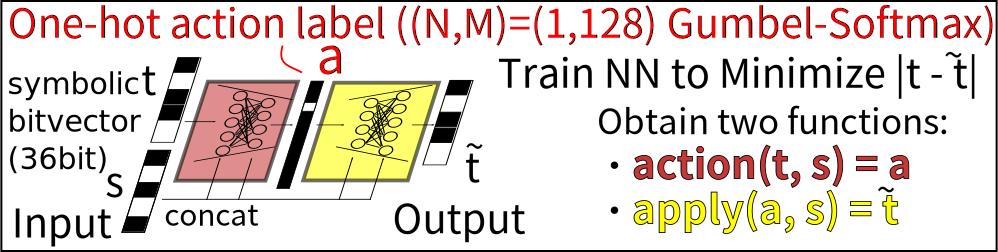
\includegraphics[width=\linewidth]{img/aae/aae.pdf}
 \caption{Action Autoencoder.}
 \label{fig:aae}
\end{figure}

To solve this, we propose an Action Autoencoder (AAE, \refig{fig:aae}). % made it more clear that the AAE is your idea, not something that's already known
The key idea of AAE is to reformulate the transitions as $apply(a,s)=t$, which lifts the action symbol and makes it trainable,
and to realize that $s$ is the \emph{background information} of the state transition function.
The AAE has $s,t$ as inputs and reconstructs $t$ as $\tilde{t}$ whose error $|t-\tilde{t}|$ is minimized.
The main difference from a typical AE is:
(1) The latent layer is a Gumbel-Softmax one-hot vector indicating the \textbf{action label} $a$. %added bf to make this def noticeable so that nobody gets confused and thinks that an action label is a human-assigned label
(2) Every layer is concatenated with $s$.
The latter conditions the entire network by $s$,
which makes the 128 action labels (7bit) represent only the \emph{conditional information} (difference) necessary to ``reconstruct $t$ \emph{given} $s$'',
unlike typical AEs which encode the \emph{entire} information of the input.
% In a typical AE, the \emph{entire} information of the input is maintained in the latent space because it can restore the original input.
% %ensuring that the information is not lost during the network flow. % "information not lost" too strong; "network flow" is a term strongly associated with combinatorial optimization
% In contrast, in our AAE, 128 action labels (7bit) represent only the \emph{conditional information} (difference) of $t$ \emph{given} $s$, as $s$ is necessary to reconstruct $t$ from $a$.
% AE learns the identity function $x=\textit{Id}(x)$, but AAE learns the \emph{conditional} identity function $t=\textit{Id}(t,s)$.
% Thus, in order to reconstruct the successor state $\tilde{t}$, it requires both the latent layer (action label) $a$ as well as the before-state $s$ acting as a conditional prior.
% 
% The before-state is only fed to the network and is not learned; 
% This means that the differences in the valid transitions can be effectively compressed into the 7-bits represented by the action labels.
As a result, the AAE learns the bidirectional mapping between $t$ and $a$, both conditioned by $s$:
\begin{itemize}
\setlength{\itemsep}{-0.3em}
 \item $Action(t,s)=a$ returns the action label from $t$.
 \item $Apply(a,s)=\tilde{t}$ applies $a$ to $s$ and returns a successor $\tilde{t}$. 
\end{itemize}

The number of labels serves as the upper bound on  the number of action symbols learned by the network.
Too few labels make AAE reconstruction loss fail to converge to zero.
After training, some labels may not be mapped to by any of the example transitions.
In the later phases of \latentplanner, these unused labels are ignored.
Since we obtain a limited number of action labels,
we can enumerate the candidates of the successor states of the given current state in constant time.
Without AAE, all $2^N$ states would be enumerated as the potential successors, which is clearly impractical.

\subsubsection{Action Discriminator}

An AAE identifies the number of actions and learns the effects of actions, but does not address the applicability (preconditions) of actions.
Preconditions are necessary to avoid invalid moves (e.g. swapping 3 tiles at once) or invalid states (e.g. having duplicated tiles), as shown in \refig{fig:aae-mixed}.
% 
Thus we need an \textit{Action Discriminator} (AD, \refig{fig:ad}) which learns the 0/1 mapping for each transition indicating whether it is valid, i.e., the ``preconditions''. This is a standard binary classification function which takes $s,t$ as inputs and returns a probability that $(s,t)$ is valid.

\begin{figure}[tbp]
 \centering
 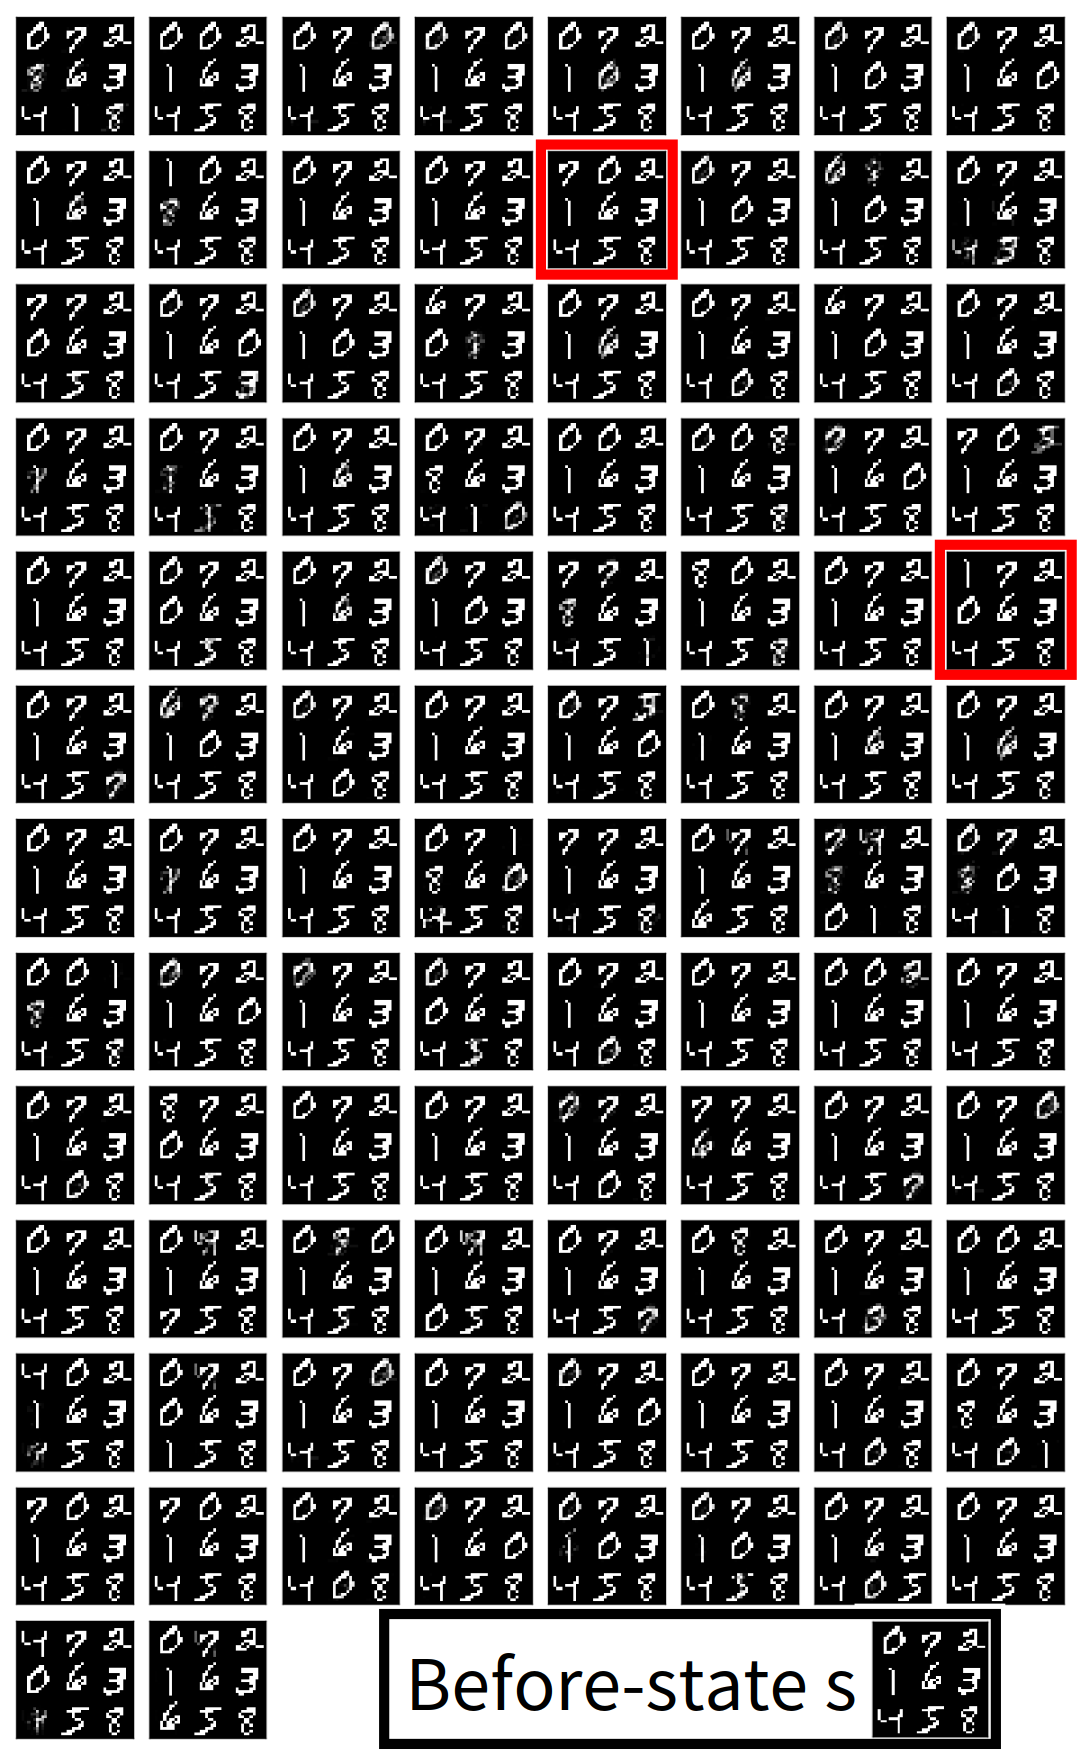
\includegraphics[width=0.8\linewidth]{img/aae/aae_mixed_states.pdf}
\caption{The successors of a state $s$ (bottom-right),
  generated by applying all 98 actions identified by the AAE.
 A valid successor is marked by the red border.}
 \label{fig:aae-mixed}
\end{figure}

\begin{figure}[tbp]
 \centering
 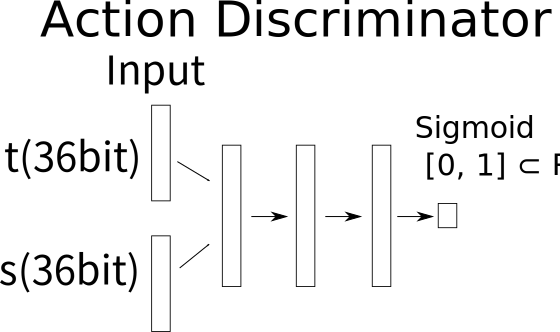
\includegraphics[width=0.5\linewidth]{img/aae/ad.pdf}
 \caption{Action Discriminator.}
 \label{fig:ad}
\end{figure}

One technical problem in training the AD is that explicit \emph{invalid} transitions are unavailable.
This is not just a matter of insufficient data, but rather a fundamental constraint in an image-based system operating in the physical environment: Invalid transitions which violate the laws of physics (e.g. teleportation) are \emph{never} observed (because they never happens).
We then might consider ``imagining/generating'' the negative examples, as humans do in a thought experiment, but it is also impossible due to the lack of specification of \emph{what} is invalid.

To overcome this issue, we use the PU-Learning framework \cite{elkan2008learning}, which can learn a positive/negative classifier from the positive and \emph{mixed} examples that may contain both positive and negative examples.
% 
We used $\overline{Tr}$ as the positive examples (they are all valid).
The mixed, i.e. possibly invalid, examples are generated by
applying each action $a$ (except unused ones) on each before-state $s$ in $\overline{Tr}$, and
removing the known positive examples from the generated pairs $(s,\tilde{t})$.

\subsubsection{PU-learning}
\label{sec:pu-learning}

The implementation of PU-learning follows \cite{elkan2008learning}.
Given a positive ($p$) and a mixed ($m$) dataset,
 $p$ and $m$ are first arbitrarily divided into a training set ($p_1$ and $m_1$)
and validation set ($p_2$ and $m_2$).
% 
Next a binary classifier for $p_1$ (true) and $m_1$ (false) is trained.
As a result, we obtain a positive/mixed classifier $d_1(x)$ which is a function which returns a probability
that a data $x$ belongs to $p_1$.
% 
After the training has finished,
the positive examples in the validation set ($p_2$) are classified, and
the  probability of $p_2$ belonging to $p_1$ are averaged to obtain a scalar $c = average(d_1(p_2))$.
% 
As the final step, the true positive/negative classifier $d_2(x)$,
which is a function which returns a probability that a data $x$ is positive,
is defined as $d_2(x) = c \cdot d_1(x)$. 

\subsubsection{State Discriminator}

As a performance improvement, we also trained a State Discriminator (SD) which is a binary classifier for a single state $s$ and detects the invalid states, e.g. states with duplicated tiles in 8-puzzles. Again, we use PU-learning. Positive examples are the before/after states in $\overline{Tr}$ (all valid). Mixed examples are generated from the random bit vectors $\rho$ (may be invalid):
Many of the images $Decode$'ed from $\rho$ are blurry and do not represent autoencodable, meaningful real-world images.
However, when they are repeatedly encoded/decoded (\refig{fig:random-bit}), they converge to the clear, autoencodable invalid states because of the denoising AE \cite{vincent2008extracting}, and we used the results as the mixed examples.
If $Decode(\rho)$ results in a blurry image,
this ``blur'' is recognized as a noise and reduced in each autoencoding step,
finally resulting in a clean, reconstructable invalid image.
We use the SD to prune some mixed action examples for the AD training so that they contain only the valid successors.
This improves the AD accuracy significantly.

\begin{figure}[tbp]
 \centering
 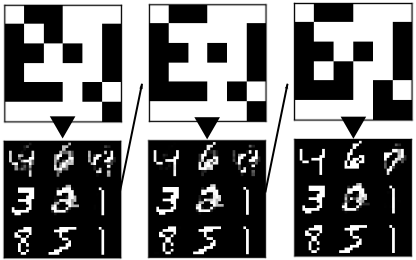
\includegraphics[width=0.5\linewidth]{img/aae/random-convergence.pdf}
 \caption{
(top, left) Random bit vector $\rho$,
(bottom, left) $Decode(\rho)$,
(top, middle)  $Encode(Decode(\rho))=\rho_2$,
(bottom, middle) $Decode(\rho_2)$,
(top, right)  $Encode(Decode(\rho_2))=\rho_3$,
(bottom, right) $Decode(\rho_3)$.
As more autoencoding is performed, images become less blurry,
 although they are still invalid (two 1-tiles).
}
\label{fig:random-bit}
\end{figure}






% \onecolumn
% \makeatletter
% \@maketitle
% \makeatother
% 
% 
% 
% \begin{landscape}
% aaa
% \end{landscape}

\fontsize{9.5pt}{10.5pt}
\selectfont
 
\bibliography{journals,confs}
\bibliographystyle{aaai}

\end{document}
